\section{Random Forests}

\subsection{Analyzing satellite data}

\subsubsection{Building, training, and evaluating the model}

In the attached \texttt{code.py}, I build and train a random forest model on the
training data using \texttt{sklearn.ensemble.RandomForestClassifier}. Below
snippet shows the most important bits:

\begin{minted}{python}
train_data = np.load(data_dir + "landsat_train" + data_extension)
train_y = train_data[:, 0]
train_X = train_data[:, 1:]
RFC = RFClassifier(n_estimators = 10,  # 10 trees in forest.
                   criterion = "gini", # use Gini impurities.
                   bootstrap = True,   # use bootstrap samples.
                   max_depth = None,   # build full trees.
                   n_jobs = -1,        # might aswell parallelize.
                   random_state = 2,   # for reproducibility.
                  )
RFC.fit(train_X, train_y)
\end{minted}

Next, I use the trained model to predict the labels for the validation set as
such:

\begin{minted}{python}
validation_data = np.load(data_dir + "landsat_validation" + data_extension)
validation_y    = validation_data[:, 0]
validation_X    = validation_data[:, 1:]

predictions = RFC.predict(validation_X)
accuracy    = np.mean(predictions == validation_y)
\end{minted}

And I find the validation accuracy to be 0.751.

\subsubsection{Plotting}

In below \cref{fig:landsat_area} I plot the predicted labels for the
\texttt{landsat\_area.csv} dataset.

\begin{figure}[H]
  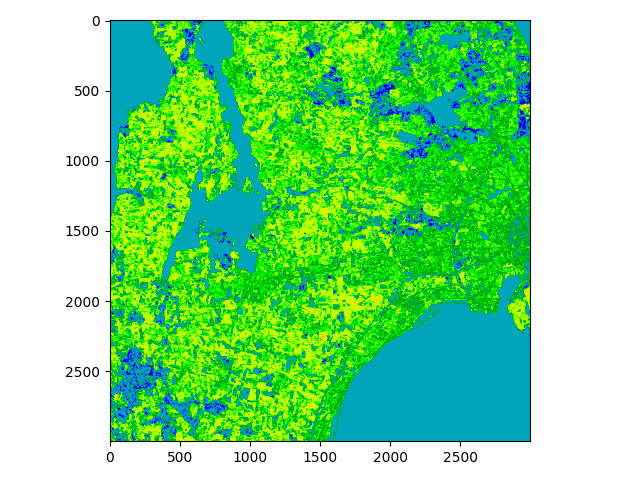
\includegraphics[width=\textwidth]{figures/landsat_area_predictions.png}
  \vspace{-0.8cm}
  \caption{\small \textit{Plot of predicted labels for the}
  \texttt{landsat\_area.csv} \textit{dataset.}}
  \label{fig:landsat_area}
\end{figure}

The plot shows a satellite image of a part of eastern Sjælland, including half
of Copenhagen, some of Amager, Roskilde, Furesø, etc.

\subsubsection{Maximum depth/height of binary decision trees}

The maximum depth/height of a binary decision tree built over $n$ training data points
is $n - 1$ (using one-based counting). This worst-case scenario occurs when at
each internal node of the tree, the decision boundary is chosen such that the
training data $S$ is split into $L_{d, \theta}$ and $R_{d, \theta}$ with:
\begin{alignat}{3}
  &|L_{d, \theta}| = 1 &&\, \text{ and }\,  |R_{d, \theta}| = |S| - 1\\[6pt]
  \text{or }\quad &|L_{d, \theta}| = |S| - 1 &&\, \text{ and }\,  |R_{d, \theta}| =
  1\, .\label{eq:norm}
\end{alignat}

As an example, consider a training set with $n = 100$ training points. At the
root node, the training set is split into two sub-trees of size 1 and 99,
respectively. The size 1 sub-tree is trivially pure and is no longer split. The
set of points in the other sub-tree is split into two new sets of size 1 and 98.
This repeats another 97 times until the 99'th split which produces two sub-trees
of size 1.

\subsection{Normalization}

\paragraph{Transformation invariance of KNN}~\smallskip

For the nearest neighbour classifier to be invariant under some transformation
$f$ of the input space, we must have that the nearest neighbour relation of points
is preserved under $f$. In other words, if we have $\text{dist}(\mbf x, \mbf y)
\leq \text{dist}(\mbf x, \mbf z)$ for some vectors $\mbf x, \mbf y, \mbf z \in
\mathbb R^n$ and a monotone distance function $\text{dist}$, then
$f$ must satisfy:

\begin{align*}
  \text{dist}(\mbf x, \mbf y) \, \leq \, \text{dist}(\mbf x, \mbf z)\quad
  \Leftrightarrow \quad
  \text{dist}(f(\mbf x), f(\mbf y)) \, \leq\, \text{dist}(f(\mbf x), f(\mbf z)).
\end{align*}

This relationship is preserved whenever $f$ is monotonic\footnote{For the case
of $n > 1$, define monotonicity as such: $f$ is monotonic if $\forall i\,:\ a_i < b_i \iff
f(\mbf a)_i < f(\mbf b)_i$.}. However, to
illustrate, let $\text{dist}$ be Euclidean distance, and $f$ be the
normalization function:

\begin{align*}
  \text{dist}(\mbf a, \mbf b) &= \sqrt{\sum_{i = 1}^n \left(a_i - b_i\right)^2}, \\[4pt]
  f(\mbf a)_i &= \frac{a_i - \mu}{\sigma},
\end{align*}

where $\mu$ and $\sigma$ are the mean and standard deviation of the input set,
respectively. Then we have:

\begin{align*}
  \text{dist}(f(\mbf a), f(\mbf b)) &= \sqrt{\sum_{i = 1}^n \left(\frac{a_i -
  \mu}{\sigma}- \frac{b_i - \mu}{\sigma}\right)^2}\\[4pt]
  &= \sqrt{\frac{1}{\sigma}\sum_{i = 1}^n \left(a_i - b_i\right)^2}\\[4pt]
\end{align*}

Since $\sigma$ is always non-negative, the square root is still defined.
Plugging this into \cref{eq:norm}:

\begin{alignat*}{3}
  &\sqrt{\sum_{i = 1}^n \left(a_i - b_i\right)^2} &&\quad \leq\quad  \sqrt{\sum_{i = 1}^n
  \left(a_i - b_i\right)^2}\\[4pt]
  \Leftrightarrow\quad  &\sqrt{\frac{1}{\sigma}\sum_{i = 1}^n \left(a_i -
  b_i\right)^2} &&\quad \leq\quad  \sqrt{\frac{1}{\sigma}\sum_{i = 1}^n \left(a_i - b_i\right)^2}
  \\[4pt]
\end{alignat*}

We see that the nearest-neighbour relation is preserved under $f$.


\paragraph{Transformation invariance of Random Forests}~\smallskip

Similar reasoning applies to the case of Random Forests. At each internal node
of each tree in the Random Forest, some comparison $a \leq b$ is made, and if
$f$ is a monotone function then $a \leq b$ again implies $f(a) \leq f(b)$.

\sectend
